% AeroGate: research-style description of the models and algorithms.
% Compile: pdflatex aerogate_paper.tex (twice), or upload to Overleaf.
% Packages used are all in a standard TeX Live / MiKTeX install.
\documentclass[11pt]{article}

\usepackage[T1]{fontenc}
\usepackage{lmodern}
\usepackage[margin=1in]{geometry}
\usepackage{amsmath,amssymb,amsthm}
\usepackage{booktabs}
\usepackage{algorithm}
\usepackage{algpseudocode}
\usepackage{enumitem}
\usepackage{microtype}
\usepackage{xcolor}
\usepackage{graphicx}
\usepackage{tikz}
\usetikzlibrary{positioning,arrows.meta}
\usepackage[hidelinks]{hyperref}

\newtheorem{proposition}{Proposition}
\newtheorem{definition}{Definition}
\theoremstyle{remark}
\newtheorem*{remark}{Remark}

\newcommand{\R}{\mathbb{R}}
\newcommand{\Z}{\mathbb{Z}}
\newcommand{\G}{\mathcal{G}}
\newcommand{\F}{\mathcal{F}}
\newcommand{\Opt}{\mathcal{O}}
\newcommand{\ind}[1]{\mathbf{1}\!\left[#1\right]}

\title{\textbf{AeroGate: Explainable, Re-optimising\\ Gate Assignment under Irregular Operations\\ at Toronto Pearson}}
\author{Shawn Wei\\ University of Waterloo\\ \small Brock Solutions Airport Innovation Challenge, subproblem 03 (gate assignment)}
\date{November 2026}

\begin{document}
\maketitle

\begin{abstract}
Irregular operations (delays, aircraft swaps, cancellations, gate outages and diversions) force gate
planners to re-plan many times a day, under hard safety rules and with little time to check a
proposal. We present \emph{AeroGate}, a rolling-horizon gate assignment system that re-solves the
whole gate plan at every information update with an exact constraint-programming model whose
objective is the evaluator's own score. Three ingredients make the plans usable in operations:
(i) \emph{move-ordering constraints} that guarantee a plan can be executed one reassignment at a time,
(ii) a \emph{safety replay} that re-checks every action with the evaluator's rules, inside a chain of
fallbacks so that the decision function never fails, and (iii) a \emph{per-decision explanation} that
records the rules each choice passed, its cost, and why every other gate lost. A realism layer for
Terminal~1 at Toronto Pearson (CYYZ), built from OpenStreetMap, adds US pre-clearance and swing gates
with security sweeps, wingtip clearance between neighbouring stands, tarmac holds priced against
Canada's three-hour APPR limit, and connecting passengers. On the 12 challenge scenarios AeroGate
has no hard failures and the lowest total score (96.2 against 104.3 and 96.8 for the provided
greedy and first-fit planners); on 40 randomly generated days it fails once (an unavoidable case)
against 3 and 6, and wins 26 of the 33 days that all planners complete. On a Pearson evening bank
it gates all 83 flights, and every re-plan after the first is proven optimal in at most 1.5~s. A
surface simulation animates the plan on the real airfield (dual arrival runways, runway crossings,
conflict-free taxiing and taxiway holding) so that operators can see, not just read, the plan.
\end{abstract}

\section{Introduction}
Gate assignment decides, for every flight, the gate (stand) it uses while on the ground. In normal
operations the schedule is planned the day before; on the day, irregular operations (IROPS) keep
invalidating it. A 40-minute delay overlaps the next aircraft at the gate; an equipment swap brings a
widebody that needs a jetbridge and a bigger stand; a jetbridge fails; a diverted aircraft arrives
with no booking. Each event triggers a re-plan, and each re-plan must (a) never break a hard rule,
(b) move as few published gates as possible, because moves cost passengers and staff, and (c) be
trusted by the person who has to approve it within minutes.

The challenge environment (the \emph{GMS evaluator}) replays a day as a sequence of updates. At each
update the solution receives the current state and returns new assignments and reassignments, which
the evaluator applies one at a time, rejecting the run if any action breaks a hard rule. The score
penalises walking distance, premium-gate use, reassignments and unassigned flights.

\paragraph{Contributions.}
\begin{enumerate}[leftmargin=*,itemsep=2pt]
\item An exact rolling-horizon CP-SAT model whose objective is the evaluator's score, re-solved over
      all flights at every update (Section~\ref{sec:model}).
\item Move-ordering constraints with integer positions that make every optimal plan executable under
      sequential application, and a no-good loop for residual cycles (Section~\ref{sec:order}).
\item A never-fail decision function: safety replay with the evaluator's own checks and a chain of
      fallbacks (Section~\ref{sec:safety}).
\item Counterfactual explanations for every decision (Section~\ref{sec:explain}).
\item A Pearson realism layer from OpenStreetMap: pre-clearance, swing gates, wingtip clearance,
      tarmac holds under APPR, connections (Section~\ref{sec:yyz}).
\item A surface simulation and display: arrival sequencing on two runways with crossings,
      rule-based conflict-free taxiing, holding on unused taxiways, and overlap-free rendering
      (Section~\ref{sec:sim}).
\end{enumerate}

\section{Related work}
Gate assignment is a well-studied variant of interval scheduling and assignment; Dorndorf et
al.~\cite{dorndorf2007} and Bouras et al.~\cite{bouras2014} survey models and objectives (walking
distance, robustness, towing, and disruption recovery). Over-constrained instances, where not every
flight can be gated, are treated by Ding et al.~\cite{ding2005}; multi-objective formulations by
Yan and Huo~\cite{yan2001}. Most work optimises a static plan. Our setting is a \emph{rolling} one
with an external executor that applies actions sequentially and fails hard, which motivates the
ordering constraints and safety replay. We use the CP-SAT solver of OR-Tools~\cite{ortools,perron2023},
whose optional interval variables and no-overlap constraints express gate occupancy directly.
Separation rules follow ICAO PANS-ATM~\cite{icao4444}; tarmac delay rules follow Canada's Air
Passenger Protection Regulations~\cite{appr}.

\section{Problem at one update}\label{sec:problem}
Time is measured in integer minutes; intervals are half-open. At an update at time $t$ the
observation gives the following.

\paragraph{Gates.} A set $\G$; each $g\in\G$ has the flight categories it may serve $Z_g$, maximum
wingspan $W_g$, jetbridge flag $J_g$, walking distance $d_g$ (metres), outage windows $\Omega_g$,
a position $\mathbf{p}_g\in\R^2$ in terminal metres, and (Pearson) a security-sweep time $\sigma_g$.

\paragraph{Flights.} A set $\F$ of decision flights; each $f$ has category $c_f$, wingspan $w_f$,
jetbridge need $j_f$, presence intervals $I_f=\{[s,e)\}$ at the airport, a current gate $\gamma_f$
(possibly none), whether its presence has begun ($a_f$), whether the airport caused its latest
change ($\phi_f$, e.g.\ a delay or swap), a priority flag $\pi^{\mathrm{prio}}_f$ (diversion,
medical), and (Pearson) minutes already waited on the tarmac $\tau_f$. Flights whose gate can no
longer change are \emph{fixed} and block their gate.

\paragraph{Hard rules.} Flight $f$ may use gate $g$ only if
\begin{equation}
c_f\in Z_g,\qquad w_f\le W_g,\qquad j_f\Rightarrow J_g,
\label{eq:compat}
\end{equation}
no interval of $f$ meets an outage of $g$, and no two aircraft overlap at a gate:
$[s_1,e_1)$ and $[s_2,e_2)$ conflict iff $s_1<e_2+\beta$ and $s_2<e_1+\beta$ for turnaround buffer
$\beta$ (0 in the challenge).

\paragraph{Score.} The evaluator charges, over the final plan,
\begin{equation}
S=\sum_{f}\Big(0.01\,d_{g(f)} + 5\,\ind{\text{domestic at intl gate}}\Big)
 + 10\,M_{\text{before}} + 50\,M_{\text{after}} + 100\,U + 300\,U_{\text{prio}},
\label{eq:score}
\end{equation}
where $M_{\text{before}}$ and $M_{\text{after}}$ count reassignments chosen by the solution before and
after the aircraft's presence began, and $U$, $U_{\text{prio}}$ count ungated regular and priority
flights. Moves forced by the airport (a flagged flight whose old gate became invalid) are not
charged. Any hard-rule violation ends the run, so it outweighs any soft saving.

\section{Optimisation model}\label{sec:model}
Figure~\ref{fig:pipeline} shows the pipeline run at every update; this section describes the model
at its centre, and Sections~\ref{sec:safety} and~\ref{sec:explain} the steps around it.

\begin{figure}[htbp]
\centering
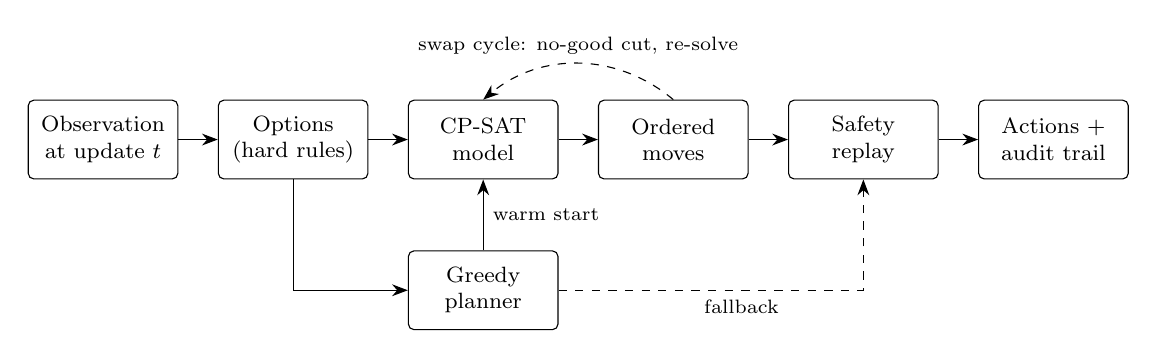
\begin{tikzpicture}[
  box/.style={draw, rounded corners=2pt, align=center, font=\footnotesize, minimum height=10mm, minimum width=19mm, inner sep=2pt},
  node distance=5mm and 5mm, >={Stealth[length=2mm]}]
\node[box] (obs) {Observation\\at update $t$};
\node[box, right=of obs] (opt) {Options\\(hard rules)};
\node[box, right=of opt] (cp) {CP-SAT\\model};
\node[box, right=of cp] (ord) {Ordered\\moves};
\node[box, right=of ord] (rep) {Safety\\replay};
\node[box, right=of rep] (out) {Actions +\\audit trail};
\node[box, below=9mm of cp] (gr) {Greedy\\planner};
\draw[->] (obs) -- (opt);
\draw[->] (opt) -- (cp);
\draw[->] (cp) -- (ord);
\draw[->] (ord) -- (rep);
\draw[->] (rep) -- (out);
\draw[->] (opt.south) |- (gr.west);
\draw[->] (gr) -- node[right, font=\scriptsize] {warm start} (cp);
\draw[->, dashed] (ord.north) to[bend right=40] node[above, font=\scriptsize] {swap cycle: no-good cut, re-solve} (cp.north);
\draw[->, dashed] (gr.east) -| node[pos=0.3, below, font=\scriptsize] {fallback} (rep.south);
\end{tikzpicture}
\caption{Decision pipeline at one update. Options already satisfy the hard rules; CP-SAT optimises the
evaluator's score with a greedy warm start; moves are ordered so they can be applied one at a time;
every action is re-checked with the evaluator's own rules before it is returned, with the greedy plan
(and then the provided reference planner) as fallbacks.}
\label{fig:pipeline}
\end{figure}

\subsection{Options}
Rather than pairing flights and gates inside the solver, we enumerate \emph{options} that already
satisfy the hard rules. For flight $f$, gate $g$ satisfying~\eqref{eq:compat} and tarmac hold
$h\in H_f$ (Pearson only; $H_f=\{0\}$ otherwise), the option $o=(f,g,h)$ has shifted presence
\begin{equation}
I_o=\big\{[s_1+h,\ \max(e_1,\ s_1+h+m_f))\big\}\cup\{I_f\setminus[s_1,e_1)\},
\end{equation}
where $[s_1,e_1)$ is the first interval and $m_f=30$ the minimum turn. Options that hit an outage or
a fixed occupancy are discarded and recorded (with the reason) for the explanation. Its occupancy on
$g$ is $P_o=\mathrm{merge}\{[s,\max(e+\beta,s+1))\}$; a flight that stays on its gate blocks the union
of its old and new intervals. Every flight that holds a gate also gets a last-resort option ``stay,
although invalid'' with cost $10^7$, so the model is always feasible.

\subsection{Variables and constraints}
Binary $x_o$ selects option $o\in\Opt_f$; binary $u_f$ marks flight $f$ ungated.
\begin{align}
\textstyle\sum_{o\in\Opt_f}x_o &= 1 && f\in\F,\ \gamma_f\ne\varnothing \label{eq:one}\\
\textstyle\sum_{o\in\Opt_f}x_o + u_f &= 1 && f\in\F,\ \gamma_f=\varnothing \label{eq:atmost}\\
\textsc{NoOverlap}\big(\{\langle P_o, x_o\rangle : o \text{ on } g\}\big) &&& g\in\G \label{eq:nooverlap}\\
x_a+x_b &\le 1 && (a,b)\in\mathcal{C}_{\text{sweep}}\cup\mathcal{C}_{\text{wing}} \label{eq:pairs}
\end{align}
Constraint~\eqref{eq:one} is an equality because the evaluator has no ``unassign'' action: a flight
that holds a gate must end on some gate. Constraint~\eqref{eq:nooverlap} uses optional fixed-size
interval variables, present iff $x_o=1$. The pair sets in~\eqref{eq:pairs} are
\begin{align*}
\mathcal{C}_{\text{sweep}} &= \{(a,b): g_a=g_b=g,\ |Z_g|\ge2,\ c_a\ne c_b,\ s_b\in[e_a,e_a+\sigma_g)\},\\
\mathcal{C}_{\text{wing}} &= \{(a,b): (g_a,g_b,L)\in\mathcal{A},\ I_a\cap I_b\ne\varnothing,\ w_a+w_b>L\},
\end{align*}
where $\mathcal{A}$ lists neighbouring gate pairs with a combined-wingspan limit $L$
(Section~\ref{sec:yyz}). Both are found with a sweep over intervals sorted by start time.

\subsection{Objective}
All costs are integers (evaluator points $\times100$). The cost of option $o=(f,g,h)$ is
\begin{equation}
c_o = d_g + 500\,\ind{\text{premium}} + 1000\,\ind{\text{move},\neg a_f,\neg\phi_f}
      + 5000\,\ind{\text{move}, a_f} + \kappa_f\,\Phi(\tau_f+h),
\end{equation}
with $\kappa_f=3$ for priority flights and 1 otherwise, and the convex tarmac-hold penalty
\begin{equation}
\Phi(t) = 20\,t + 0.9\,U_0\,(t/180)^4,\qquad U_0=10\,000,
\label{eq:hold}
\end{equation}
which is cheap for short holds and climbs steeply toward the 180-minute APPR limit (options beyond
it are not generated). An ungated flight costs $U_f = 10\,000$ ($30\,000$ if priority) plus
$\Phi(\tau_f)$ if it is already waiting. Connecting passengers $(a,d,n)$ add a walking term: integer
positions $X_f,Y_f$ are tied to the chosen gate by $x_o \Rightarrow (X_f,Y_f)=\mathbf{p}_{g_o}$, and
\begin{equation}
\min\ \sum_{o}c_o x_o + \sum_f U_f u_f + \sum_{(a,d,n)} \lceil \rho n \rceil\big(|X_a-X_d|+|Y_a-Y_d|\big),
\label{eq:obj}
\end{equation}
with the absolute values linearised by CP-SAT's \texttt{AddAbsEquality}. Without the Pearson-only
tarmac-hold and connection terms, \eqref{eq:obj} equals $100\,S$ in~\eqref{eq:score} on the decision
flights, so the
solver only moves a published gate when the move saves more than it costs. Weights are read live
from the evaluator's configuration, so a re-tuned evaluator is followed automatically.

\subsection{Move ordering}\label{sec:order}
The evaluator applies reassignments one by one, each checked against the gates \emph{as they are at
that moment}. A plan that swaps two flights (A to B's gate, B to A's gate) is optimal but cannot be
applied. Let $\mathcal{M}=\{f:\gamma_f\ne\varnothing\}$ and introduce integer positions
$\pi_f\in\{0,\dots,|\mathcal{M}|\}$. For every option $o$ that moves $f$ onto a gate currently held by
$b\ne f$ with overlapping intervals,
\begin{equation}
x_o \Rightarrow \pi_b + 1 \le \pi_f.
\label{eq:order}
\end{equation}

\begin{proposition}
In any solution of \eqref{eq:one}--\eqref{eq:order}, applying the reassignments in increasing order of
$\pi$ never moves a flight onto a gate still held, at an overlapping time, by a flight that has not
moved yet.
\end{proposition}
\begin{proof}
Suppose $f$ moves onto gate $g$ held by $b$ with overlapping intervals. Then~\eqref{eq:order} gives
$\pi_b<\pi_f$, so $b$ is processed first. If $b$ stays on $g$, its option and $f$'s option both
occupy $g$ at overlapping times, contradicting~\eqref{eq:nooverlap}; so $b$ moves away first. A
cycle $f_1\to\dots\to f_k\to f_1$ of such dependencies would require
$\pi_{f_1}<\pi_{f_2}<\dots<\pi_{f_1}$, which is impossible.
\end{proof}

The occupancy the evaluator checks at application time can differ slightly from the model's (e.g.\
a flagged flight's old booking), so the action builder sorts the moves topologically and, if a
residual cycle remains, adds the no-good $\bigvee_{(f,g)\in\text{cycle}}\neg x_{f,g}$ and re-solves (at
most eight times, then falls back to the greedy plan).

\subsection{Solving}
CP-SAT runs with one search worker, a fixed random seed and a \emph{deterministic} time budget
(2.0 deterministic seconds per update; 2.5 in the Pearson layer), with the wall clock only as a
safety net. The same input therefore yields the same plan on every run, which matters for
explanations and for audit. The greedy plan of Algorithm~\ref{alg:greedy} is passed as a solution
hint (warm start) and is also the fallback if OR-Tools is missing or fails.

\begin{algorithm}[htbp]
\caption{Greedy planner (warm start and fallback)}\label{alg:greedy}
\begin{algorithmic}[1]
\State $B\gets$ empty board (checks overlap, sweep and wingtip rules incrementally)
\For{$f$ with $\gamma_f\neq\varnothing$} \State place the stay option of $f$ on $B$ if it exists \EndFor
\For{flagged $f$ in order of first presence}
  \State remove $f$ from $B$; if its stay option still fits, keep it
  \State otherwise place the cheapest option of $f$ that fits (or the last-resort option)
\EndFor
\State sort waiting flights by (priority first, longest tarmac wait, fewest options, earliest)
\For{each waiting $f$} \State place the cheapest option that fits, or leave $f$ ungated \EndFor
\end{algorithmic}
\end{algorithm}

\section{Execution safety}\label{sec:safety}
A hard failure ends an evaluator run, so the decision function must not fail in any way. Algorithm
\ref{alg:decide} shows the per-update pipeline.

\begin{algorithm}[htbp]
\caption{Decision at one update}\label{alg:decide}
\begin{algorithmic}[1]
\Function{Decide}{observation}
  \State $P\gets$ problem from the observation (weights read from the evaluator)
  \Repeat \Comment{at most 8 rounds}
    \State plan $\gets$ CP-SAT with cuts (greedy hint); actions $\gets$ ordered moves
    \State if a residual swap cycle exists, add a no-good cut
  \Until{no cycle}
  \State kept, errors $\gets$ \Call{Replay}{actions} \Comment{the evaluator's own compatibility and overlap checks}
  \If{errors} \State use the greedy plan instead if its replay has fewer errors \EndIf
  \State record the explanation (never allowed to raise)
  \State \Return kept
\EndFunction
\State on any exception: the provided reference planner, replayed; on a further exception: no actions
\end{algorithmic}
\end{algorithm}

\textsc{Replay} simulates the evaluator's state transitions with its own compatibility code and drops
any action that would be rejected, so the output contains only actions the evaluator accepts. Combined
with the fallbacks, the function always returns and never returns an invalid action.

\section{Explanations}\label{sec:explain}
Operators approve plans they can check. For every decision AeroGate records (a) the rules the chosen
option passed, with the numbers (``wingspan 60~m within gate limit 65~m'', ``wingtip clearance with
F62: combined 96~m $\le$ 100~m''); (b) the cost breakdown in evaluator points; and (c) a verdict for
\emph{every other gate}, by evaluating the counterfactual option $o'=(f,g')$ against the final plan:
\begin{itemize}[leftmargin=*,itemsep=1pt]
\item \textbf{rule}: $o'$ was never generated; the failed rule of~\eqref{eq:compat}, an outage, or a fixed occupancy is quoted;
\item \textbf{busy}: $o'$ is legal but conflicts in the final plan with a named flight
      (overlap~\eqref{eq:nooverlap}, sweep or wingtip pair~\eqref{eq:pairs});
\item \textbf{costlier}: $o'$ is feasible but $\Delta=c_{o'}-c_o>0$; $\Delta$ and its main driver
      (e.g.\ ``+0.90 pts: longer walk, 490~m vs 400~m'') are reported.
\end{itemize}
The dashboard shows these per flight, colours the gates on the map accordingly, and summarises each
update in plain language (``moved D51/F51 to D39 because of a delay; re-planned before landing, so no
charge''); Figure~\ref{fig:dashboard} shows one decision.

\begin{figure}[!t]
\centering
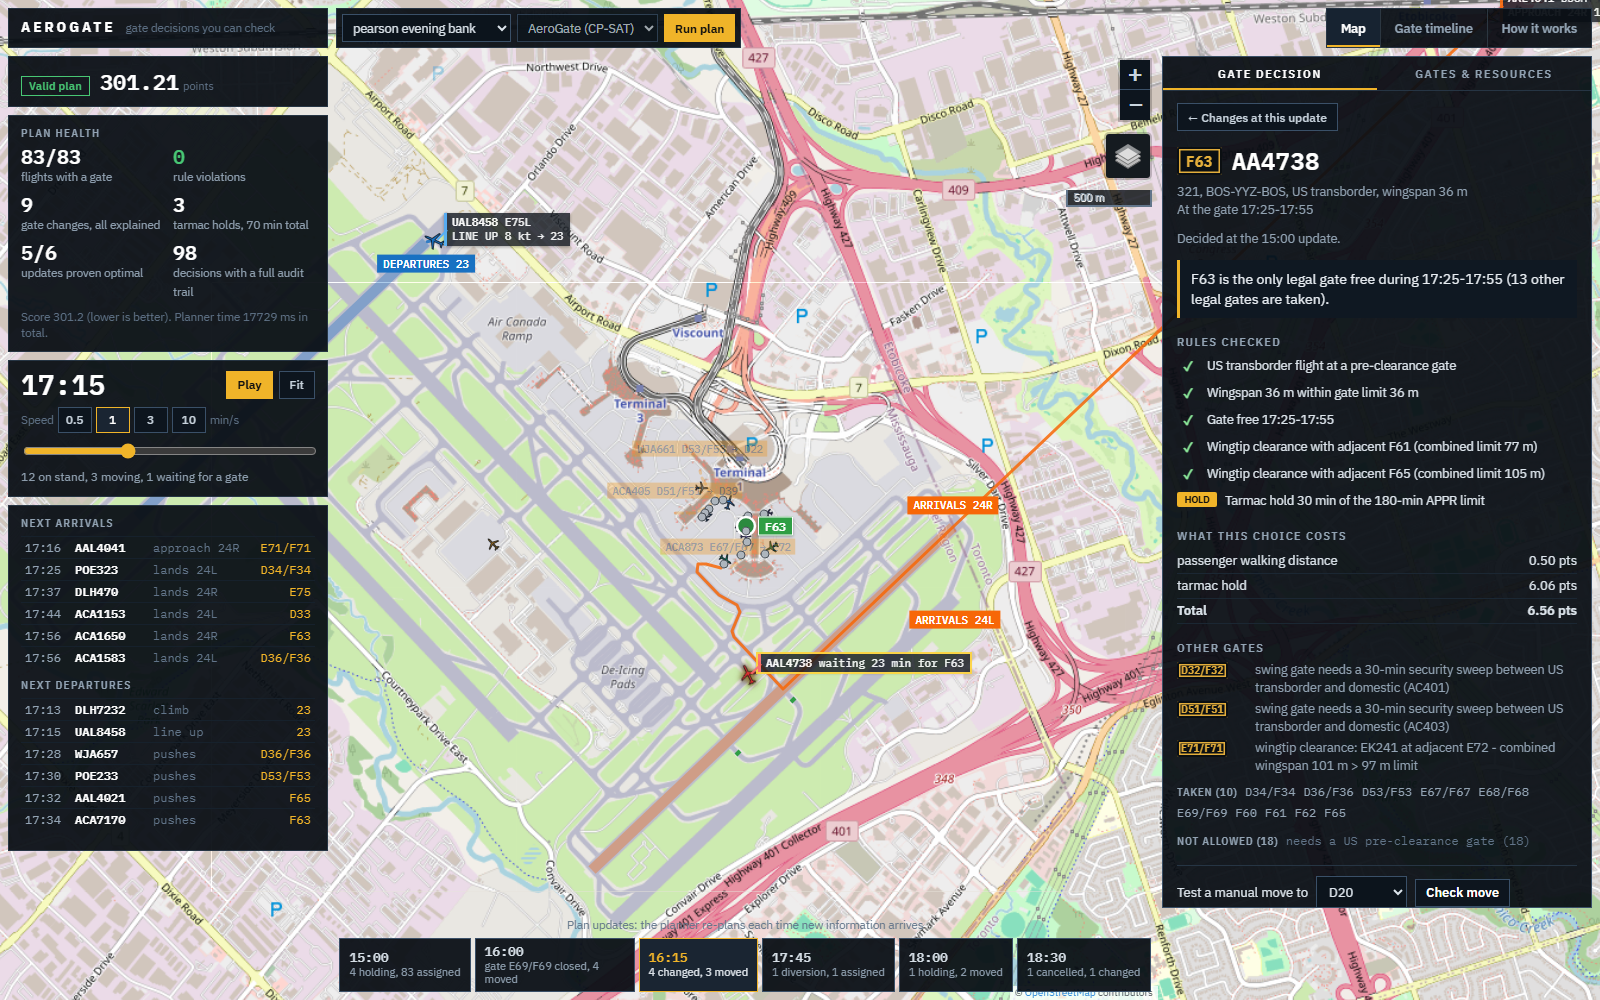
\includegraphics[width=\textwidth]{figs/dashboard_hold.png}
\caption{The operator dashboard on the Pearson evening bank at 17:15. AA4738 (US transborder A321)
holds on a taxiway holding spot for its only free legal gate, F63; its route to the stand is drawn.
The right panel is the decision record: the rules F63 passed with their numbers, the cost in
evaluator points (walking 0.50, tarmac hold 6.06), the alternatives blocked by swing-gate sweeps or
wingtip clearance, and one-line summaries of the gates that were taken or not allowed.}
\label{fig:dashboard}
\end{figure}

\section{Pearson realism layer}\label{sec:yyz}
The challenge data knows only cargo, domestic and international. We built a second model of Terminal~1
at Toronto Pearson (30 contact gates and two Cargo West stands) from an OpenStreetMap extract
\cite{osm}.

\paragraph{Geometry.} Gate names (including dual-named swing gates such as E67/F67), stand centrelines
and nose-in headings come from OSM. A stand is widebody-capable if its centreline is at least 100~m
long or it has MARS sub-stands. Walking distance is $d_g=1.3\,\lVert\mathbf{p}_g-\mathbf{c}\rVert$
from the terminal centre $\mathbf{c}$, rounded to 10~m.

\paragraph{Wingtip clearance.} Two aircraft side by side need half their spans plus a clearance
margin between centrelines: $(w_1+w_2)/2+7.5\le\delta$. Probing each stand 40~m from the nose and
measuring the spacing $\delta<75$~m to its neighbour gives the combined-span limit
\begin{equation}
L = \max\big(76,\ \mathrm{round}(2(\delta-7.5))\big),
\end{equation}
kept when $L<130$~m (24 pairs). The floor of 76~m keeps two narrowbodies abreast legal where OSM
lines converge at pier corners.

\paragraph{Operational rules.} US transborder flights need pre-clearance gates (Pier F and the D/F,
E/F swing gates); a swing gate needs a $\sigma_g=30$-minute security sweep between flights of
different zones; an arrival with no free gate may hold on the tarmac for $h\in\{0,10,20,30,60,90,
120,180\}$ minutes priced by~\eqref{eq:hold}, three times higher for medical diversions; connecting
passengers add $0.02$ points per passenger per 100~m of Manhattan distance between the two gates.

\paragraph{Scenario.} An evening bank (83 flights, six updates from 15:00 to 18:30) with a jetbridge
failure on swing gate E69/F69, a thunderstorm bunching seven arrivals, a 777 medical diversion, a
787 swap on a US flight and a cancellation.

\section{Surface simulation and display}\label{sec:sim}
The optimiser decides gates and times; the dashboard animates the result on the real airfield so
operators can see congestion and conflicts. The simulation is for validation and display only; it
does not feed back into the plan.

\subsection{Runways and arrival sequencing}
Pearson's usual west-flow configuration is used: arrivals on 24R and 24L, departures from 23. Taxi
routes are shortest paths (Dijkstra~\cite{dijkstra1959}) on the OSM taxiway graph (3{,}251 nodes,
3{,}682 edges) with runway edges weighted $\times12$, so routes cross runways but never use them as
taxiways. For each gate and landing runway $r$ the exit is the junction 1.1--2.7~km down the runway
that minimises taxi length $\ell_r$. The plan's gate-in time $G_f$ gives a touchdown target per runway
\begin{equation}
t^0_{f,r} = G_f - h_f - R - \ell_r/v_{\text{taxi}} - \ell_{\text{entry}}/v_{\text{stand}},
\end{equation}
with roll-out $R=1.1$~min, $v_{\text{taxi}}=480$~m/min and $v_{\text{stand}}=110$~m/min. Arrivals are
taken in order of $\min_r t^0_{f,r}$ and each is given the runway minimising its lateness
$t_{f,r}-t^0_{f,r}$ (ties: the runway idle longest), where
\begin{equation}
t_{f,r} = \max\Big(t^0_{f,r},\ t_{\text{prev}(r)} + \max\big(\tfrac{60\,s(\text{prev},f)}{140},\,1.4,\,X_r\big),\ t_{\text{last}}+0.65\Big).
\end{equation}
Here $s\in\{3,4,5\}$~NM is the wake separation (3 behind a medium, 4 for a heavy behind a heavy, 5
for a medium behind a heavy) flown at 140~kt, $0.65$~min staggers landings on the two close parallels (about
1.5~NM diagonal), and $X_r=2.6$~min on a runway that other traffic must cross, else 0.

\paragraph{Runway crossings.} The 24L arrivals reach Terminal~1 by crossing 24R at the same two
junctions where 24R arrivals exit. A crossing is allowed at time $T$ only if no 24R arrival has
$T>t-0.8$ (within about 2~NM of touchdown) without having already turned off and moved 120~m clear.
A landing therefore blocks crossings for roughly $0.8+1.1+0.25\approx2.15$~min; spacing 24R landings
at least $X_r=2.6$~min apart leaves a gap of at least $0.45$~min after every landing, so crossing
traffic cannot be starved.

\subsection{Ground movement}
Ground traffic is a time-stepped simulation with $\Delta t=3$~s. Each aircraft follows its route and
obeys rules designed so that every stop eventually clears:
\begin{enumerate}[leftmargin=*,itemsep=1pt]
\item stop 105~m behind an aircraft ahead in the same direction, looking 120~m ahead along the route
      so a merge onto another aircraft's taxiway is seen before the two are alongside;
\item at crossings and head-on, the aircraft that started later steps to a parallel lane 60~m to the
      side, choosing the side by where the two will be closest and never within 45~m of a parked
      aircraft; a stopped aircraft keeps its lane;
\item one pushback at a time per alley, only when no aircraft is about to pass behind the stand;
\item departures queue nose to tail at the runway 23 holding point and take off 1.5~min apart (2~min
      behind a heavy);
\item an arrival whose stand is still occupied waits where it is clear of that stand's taxi-out
      route, so the departing aircraft can get past.
\end{enumerate}

\paragraph{Holding on unused taxiways.} An aircraft that must wait for its gate (a planned tarmac
hold, or a stand that is still occupied) should not stop on the busy apron. Holding spots are the
taxiway nodes $v$ with
\begin{equation}
\mathrm{dist}(v,\text{routes})\ge80\text{ m},\quad \mathrm{dist}(v,\text{stands})\ge80\text{ m},\quad
\mathrm{dist}(v,\text{runways})\ge150\text{ m},
\end{equation}
on the terminal side of every runway, chosen greedily nearest the arrival flow with 150~m spacing (10
spots). The browser runs Dijkstra from each spot over the same graph. The simulation runs twice: the
first pass finds the arrivals that would wait for their stand for 45~s or more; the second books each
waiting aircraft onto the spot with the shortest detour $\ell(\text{exit}\to v)+\ell(v\to\text{stand})$
subject to: the spot is free for the hold interval (taken from the first pass, with margins), its
route passes no spot occupied at that time (70~m), and the spot lies on no other booked route while
it is in use.

\subsection{Overlap-free rendering}
Zoomed out, true-size aircraft are a few pixels wide; drawing them larger keeps them visible but
makes neighbours overlap. Each aircraft $i$ is drawn at scale $k_i\in[0.8,k_i^{\max}]$, where
$k_i^{\max}=\max(1, \ell^{\min}/(\text{span}_i/m))$, $m$ is metres per pixel and $\ell^{\min}$ is 17~px
(12~px parked). The plane shape $A_i(k)$ is approximated by three oriented rectangles (fuselage, wing,
tail). For each close pair, $s_{ij}$ is the largest value on a ladder of scales such that $A_i(\min(s,
k_i^{\max}))$ and $A_j(\min(s,k_j^{\max}))$ are disjoint for every ladder value up to $s$ (tested with
the separating-axis theorem), and
\begin{equation}
k_i=\min\Big(k_i^{\max},\ \min_j s_{ij}\Big),
\end{equation}
followed by a repair pass that shrinks the larger icon of any pair that still touches. Neighbours that
would touch even at true size (wingtips at corner stands) are drawn up to 20\% smaller.

\subsection{Ground crew and baggage (estimates, display only)}
Per pier $p$, ramp-crew demand is $C_p(T)=\sum_f n_f\,\ind{T\in W_f}$ with $n_f=2$ for a widebody and
1 otherwise, where $W_f$ covers 25~min after in-block (40 widebody) and 35~min before off-block (50
widebody) to 5~min after. Baggage load is $B_p(T)=\sum_f b_f/\lvert V_f\rvert\,\ind{T\in V_f}$ bags per
hour, with $b_f$ = seats $\times$ load factor $\times$ bags per passenger, unloaded over 45~min after
in-block and made up over 150~min before off-block, against belts of 1{,}200 bags/h. Staffing (D 14,
F 6, E 16, cargo 2 crews) and belts (D 2, F 1, E 4) are estimates; the planner does not use them.

\section{Results}\label{sec:results}
\begin{table}[htbp]
\centering
\caption{Evaluator results (lower score is better). Generated days use random layouts of 6--40 gates
and 12--90 flights with delays, swaps, cancellations, reinstatements, outages and diversions announced
30--180~min ahead.}
\label{tab:bench}
\begin{tabular}{lrrr}
\toprule
 & AeroGate & Provided greedy & Provided first-fit\\
\midrule
12 challenge scenarios, total score & \textbf{96.2} & 104.3 & 96.8\\
Hard failures, challenge scenarios & \textbf{0} & 0 & 0\\
40 generated days, hard failures & \textbf{1} & 3 & 6\\
Total score, 33 days all planners finish & \textbf{3{,}188} & 3{,}565 & 5{,}783\\
Days won outright (of 33) & \textbf{26} & 5 & 0\\
\bottomrule
\end{tabular}
\end{table}

\paragraph{Benchmarks.} Table~\ref{tab:bench} summarises the evaluator runs. Every generated day passes
the same guarantee as the official scenarios: after each update all active flights can be placed at
once. The one AeroGate failure (\texttt{gen\_022}) cannot be avoided by any planner: an outage hits a
parked widebody while all seven compatible gates hold parked aircraft, and the evaluator cannot swap
two parked aircraft.

\paragraph{Ablation.} A robustness bonus for slack between consecutive turns (a tight-turn penalty
linear in the gap within a 45-minute window) made the total on generated days worse (3{,}582 vs
3{,}078 at the time of the test): delays are announced before arrival, and the evaluator lets a delayed
flight move for free then, so slack bought in advance is mostly wasted. It is switched off.

\begin{table}[htbp]
\centering
\caption{Pearson evening bank: plan and per-update solve.}
\label{tab:yyz}
\begin{tabular}{lrrrr}
\toprule
Update & CP-SAT status & Solve (ms) & Decisions & Gate moves\\
\midrule
15:00 (initial plan) & feasible & 9{,}327 & 83 & 0\\
16:00 gate E69/F69 closed & optimal & 1{,}078 & 4 & 4\\
16:15 storm, delays & optimal & 1{,}500 & 7 & 3\\
17:45 medical diversion & optimal & 466 & 1 & 0\\
18:00 787 swap, hold & optimal & 622 & 2 & 2\\
18:30 cancellation & optimal & 372 & 1 & 0\\
\bottomrule
\end{tabular}
\end{table}

\paragraph{Pearson.} All 83 flights are gated with no rule violation; the score is 301.21 points
(walking 223.30, three charged moves 30.00, connecting passengers 29.79, tarmac holds 18.12).
Table~\ref{tab:yyz} gives the per-update solve: the initial 83-flight plan uses the full deterministic
budget, and every re-plan after it is proven optimal in at most 1.5~s.

\paragraph{Against greedy rules on the same evening.} To isolate the value of optimisation we re-ran
the Pearson evening with identical rules, options and disruptions, but with the greedy planner of
Algorithm~\ref{alg:greedy} alone: keep every gate, re-fit what breaks, give each waiting flight the
first good free gate. This is how rule-based tools (and a busy planner) re-plan. Table~\ref{tab:vs}
compares the two. Both gate every flight without a rule violation; the difference is the tarmac.
Looking at the whole evening at once, AeroGate spends three charged gate moves to avoid holds the
greedy rules cannot see coming, cutting held passenger-hours by 82\% and the score by 20\%.

\begin{table}[htbp]
\centering
\caption{Pearson evening bank, same rules and disruptions: AeroGate against greedy rules (no
optimisation). Passenger-hours assume an 85\% load factor.}
\label{tab:vs}
\begin{tabular}{lrr}
\toprule
 & AeroGate & Greedy rules\\
\midrule
Flights with a gate & 83/83 & 83/83\\
Rule violations & 0 & 0\\
Flights held on the tarmac & \textbf{3} & 11\\
Minutes held on the tarmac & \textbf{70} & 320\\
Passenger-hours held on the tarmac & \textbf{234} & 1{,}320\\
Gate changes & \textbf{9} & 10\\
Score (lower is better) & \textbf{301.2} & 377.9\\
\bottomrule
\end{tabular}
\end{table}

\paragraph{Surface simulation.} Over the whole evening, sampled every 6~s: 33 landings on 24R and 32
on 24L; all 76 departures from 23; no aircraft is ever on a runway while another lands on it; two 24L
arrivals hold short of 24R (at most 1.5~min); every aircraft waiting for a gate waits on a taxiway
holding spot; the closest approach between two moving aircraft is 39~m, and drawn aircraft never
overlap at 1, 3.5 or 4.9 metres per pixel.

\section{Discussion and limitations}
The exact model is small enough to re-solve the whole day at every update, which removes the usual
trade-off between local repair and global quality: the solver sees every knock-on effect of a move.
Equality with the evaluator's score makes the plan's cost auditable, and the explanation turns the
solver's choice into statements an operator can verify.

\paragraph{Limitations.} The evaluator has no ``unassign'' or remote-stand action, so some outage cases
cannot be saved (a real system would tow to a remote stand; the Pearson layer can hold on the tarmac).
Stand sizes, walking distances, crews and baggage figures in the Pearson layer are estimates. The
surface simulation is rule-based and does not optimise taxi routes or runway sequences jointly with
gates. The first plan of a large day uses the full single-thread budget.

\paragraph{Future work.} Learning delay distributions from A-CDM milestones (TOBT/TSAT) to price
buffers by probability; warm-starting from the previous update's plan; joint gate, ground-crew and
baggage optimisation using the pier estimates as constraints; and solving per pier in parallel.

\section{Conclusion}
AeroGate treats gate re-planning as a sequence of exact optimisations whose objective is the score
that judges the plan, whose output is guaranteed executable and valid, and whose every decision comes
with its reasons. On the challenge benchmarks it is never worse on hard failures and best on total
score, and on a realistic Pearson evening it keeps every flight gated while proving its re-plans
optimal in about a second.

\begin{thebibliography}{9}
\bibitem{dorndorf2007} U.~Dorndorf, A.~Drexl, Y.~Nikulin, E.~Pesch.
  Flight gate scheduling: State-of-the-art and recent developments.
  \emph{Omega}, 35(3):326--334, 2007.
\bibitem{bouras2014} A.~Bouras, M.~A.~Ghaleb, U.~S.~Suryahatmaja, A.~M.~Salem.
  The airport gate assignment problem: A survey.
  \emph{The Scientific World Journal}, 2014:923859, 2014.
\bibitem{ding2005} H.~Ding, A.~Lim, B.~Rodrigues, Y.~Zhu.
  The over-constrained airport gate assignment problem.
  \emph{Computers \& Operations Research}, 32(7):1867--1880, 2005.
\bibitem{yan2001} S.~Yan, C.-M.~Huo.
  Optimization of multiple objective gate assignments.
  \emph{Transportation Research Part A}, 35(5):413--432, 2001.
\bibitem{ortools} L.~Perron, V.~Furnon. OR-Tools. Google, \url{https://developers.google.com/optimization}.
\bibitem{perron2023} L.~Perron, F.~Didier, S.~Gay. The CP-SAT-LP solver.
  In \emph{Principles and Practice of Constraint Programming (CP 2023)}, LIPIcs 280, 2023.
\bibitem{icao4444} ICAO. \emph{Procedures for Air Navigation Services: Air Traffic Management} (Doc 4444).
\bibitem{appr} Canada. \emph{Air Passenger Protection Regulations}, SOR/2019-150.
\bibitem{dijkstra1959} E.~W.~Dijkstra. A note on two problems in connexion with graphs.
  \emph{Numerische Mathematik}, 1:269--271, 1959.
\bibitem{osm} OpenStreetMap contributors. Map data available under the Open Database License,
  \url{https://www.openstreetmap.org}.
\end{thebibliography}

\end{document}
